We explored the predicates learned by our systems qualitatively by looking at the differences in individual predicate classifier agreements, the objects picked out by these classifiers in each system, and correlations between predicate decisions and physical properties of objects.

\textbf{When multi-modal helps.} We performed a pairwise comparison of predicates built in the \textbf{multi-modal} and \textbf{vision only} systems, again using leave-one-out cross validation over objects to measure performance.
Table~\ref{tab:predicate_examples} shows the predicates for which the difference in $f_1$ between the two systems was high.

\begin{table*}
\centering
\begin{tabular}[t]{| c | c || >{\centering\arraybackslash}m{\pictablew} | >{\centering\arraybackslash}m{\pictablew} | >{\centering\arraybackslash}m{\pictablew} || >{\centering\arraybackslash}m{\pictablew} | >{\centering\arraybackslash}m{\pictablew} | >{\centering\arraybackslash}m{\pictablew} |}
	\hline
	\bf Predicate & $f_1^{mm}-f_1^{vo}$ & \multicolumn{3}{c||}{\bf High Confidence Positive} & \multicolumn{3}{c|}{\bf High Confidence Negative} \\ \hline \hline
	\multicolumn{2}{|c|}{} & \multicolumn{6}{c|}{\bf multi-modal system} \\ \hline
	can & 0.857 & 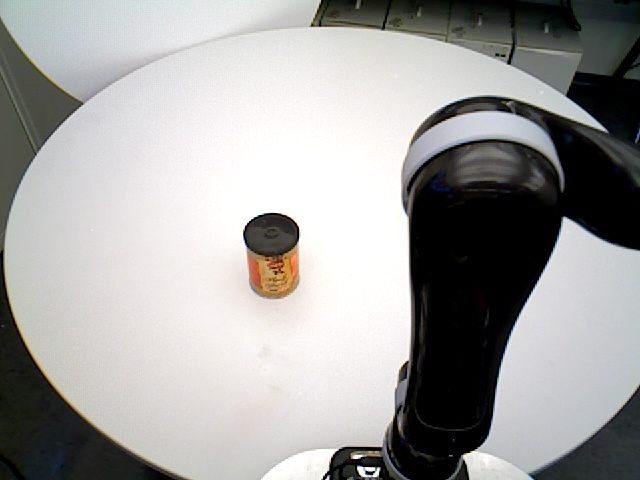
\includegraphics[scale=\examplepicsize]{figures/objects/3.JPG} & 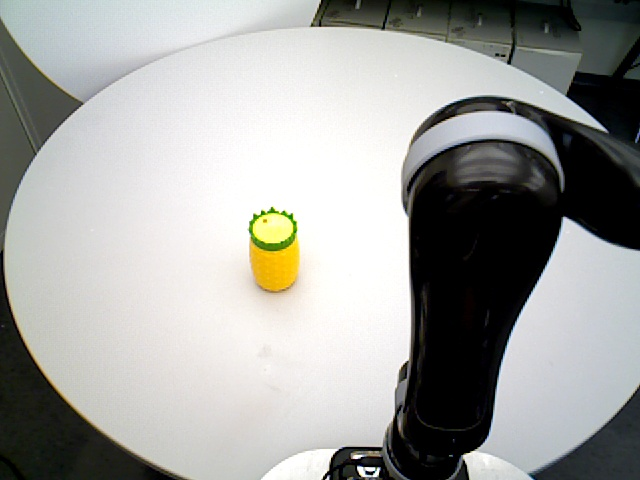
\includegraphics[scale=\examplepicsize]{figures/objects/5.JPG} & 
\includegraphics[scale=\examplepicsize]{figures/objects/6.JPG} & 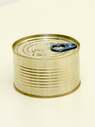
\includegraphics[scale=\examplepicsize]{figures/objects/30.JPG} & 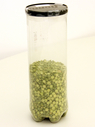
\includegraphics[scale=\examplepicsize]{figures/objects/28.JPG} & 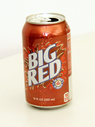
\includegraphics[scale=\examplepicsize]{figures/objects/15.JPG}\\ \hline
	tall & 0.516 & 
\includegraphics[scale=\examplepicsize]{figures/objects/22.JPG} & 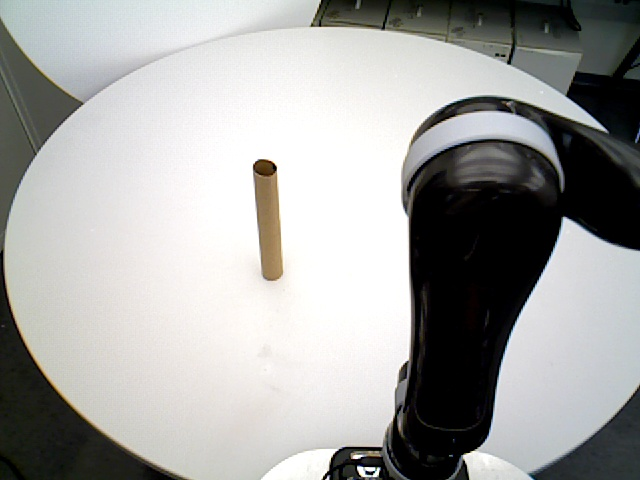
\includegraphics[scale=\examplepicsize]{figures/objects/4.JPG} & 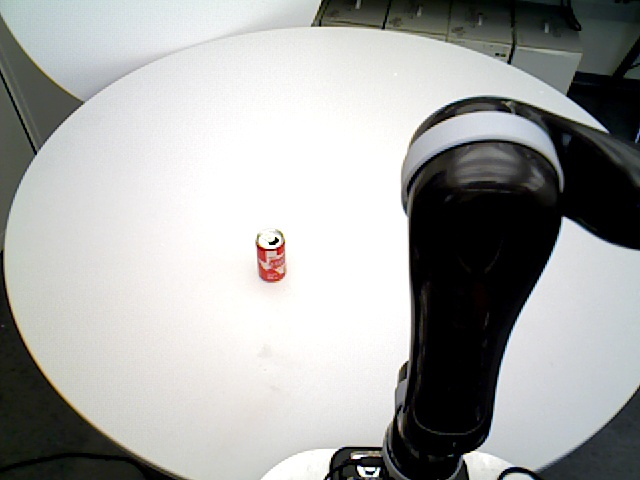
\includegraphics[scale=\examplepicsize]{figures/objects/27.JPG} & 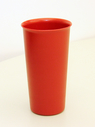
\includegraphics[scale=\examplepicsize]{figures/objects/7.JPG} & 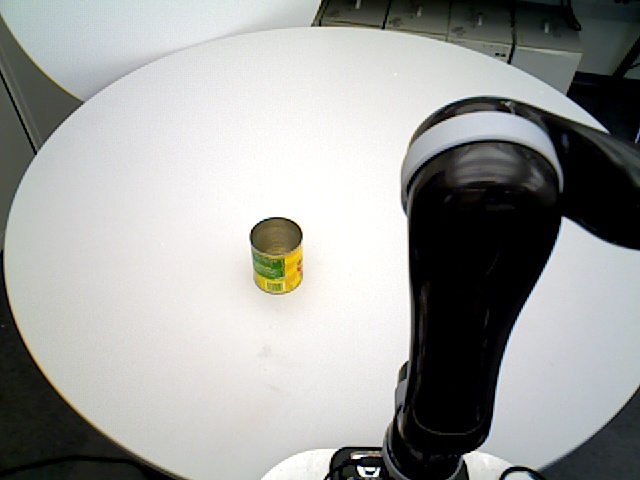
\includegraphics[scale=\examplepicsize]{figures/objects/12.JPG} & 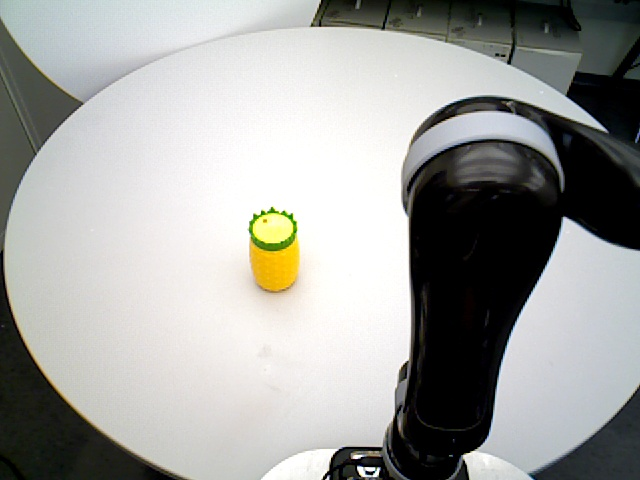
\includegraphics[scale=\examplepicsize]{figures/objects/5.JPG}\\ \hline
	half-full & .462 & 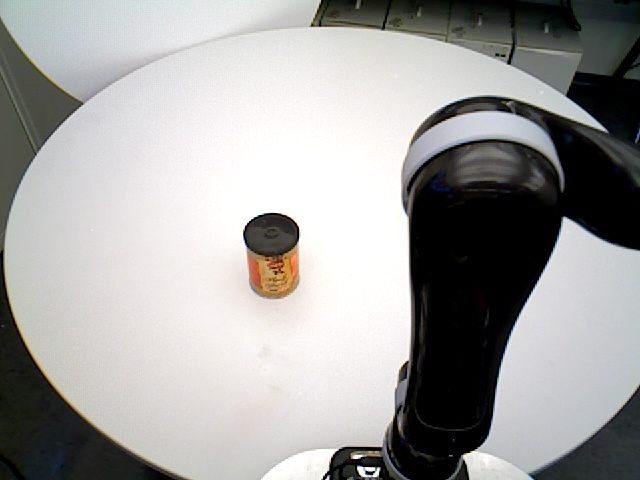
\includegraphics[scale=\examplepicsize]{figures/objects/3.JPG} & 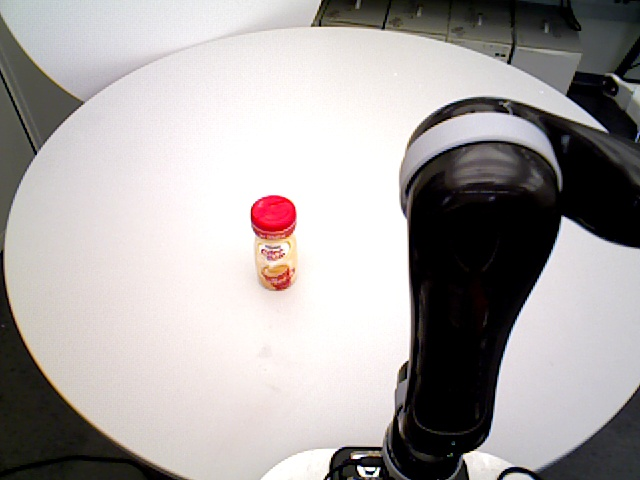
\includegraphics[scale=\examplepicsize]{figures/objects/17.JPG} & 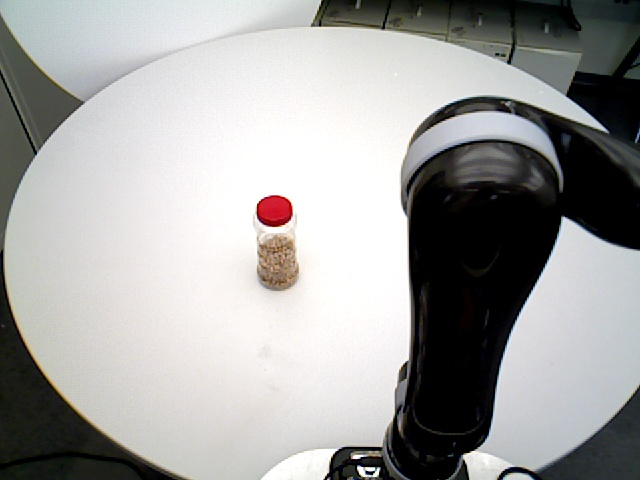
\includegraphics[scale=\examplepicsize]{figures/objects/23.JPG} & 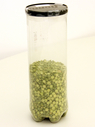
\includegraphics[scale=\examplepicsize]{figures/objects/28.JPG} & 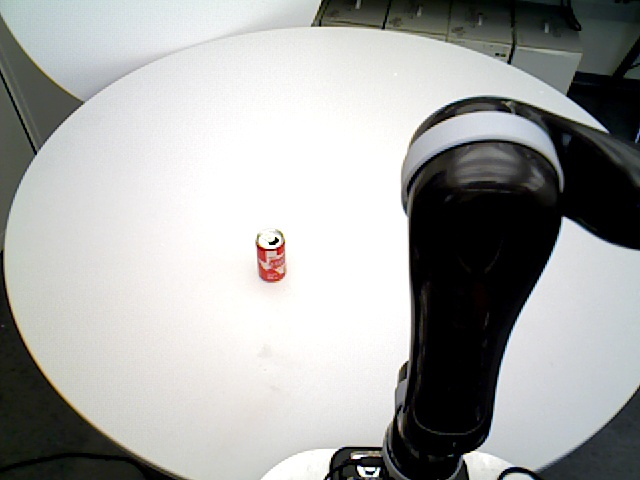
\includegraphics[scale=\examplepicsize]{figures/objects/27.JPG} & 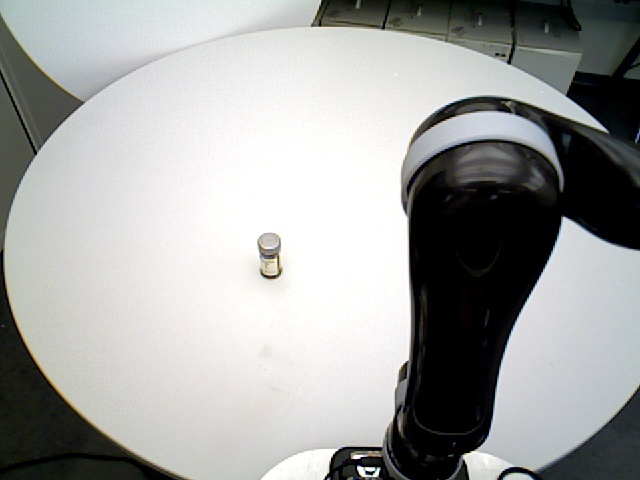
\includegraphics[scale=\examplepicsize]{figures/objects/26.JPG}\\ \hline
	yellow & .312 & 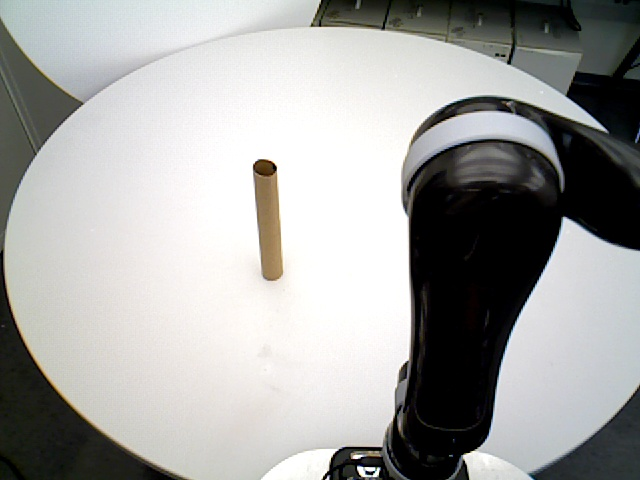
\includegraphics[scale=\examplepicsize]{figures/objects/4.JPG} & 
\includegraphics[scale=\examplepicsize]{figures/objects/6.JPG} & 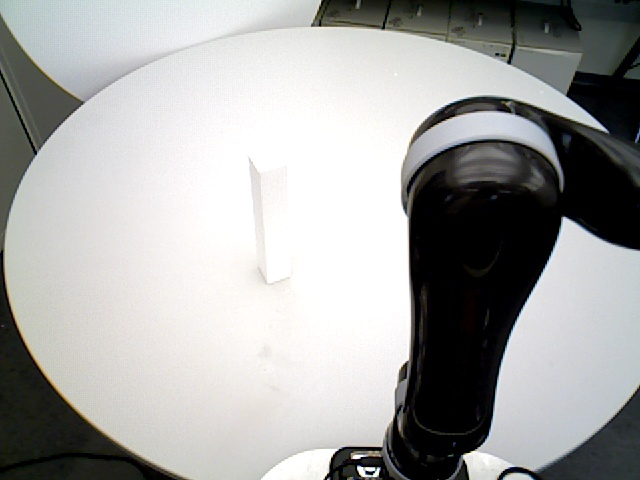
\includegraphics[scale=\examplepicsize]{figures/objects/29.JPG} & 
\includegraphics[scale=\examplepicsize]{figures/objects/18.JPG} & 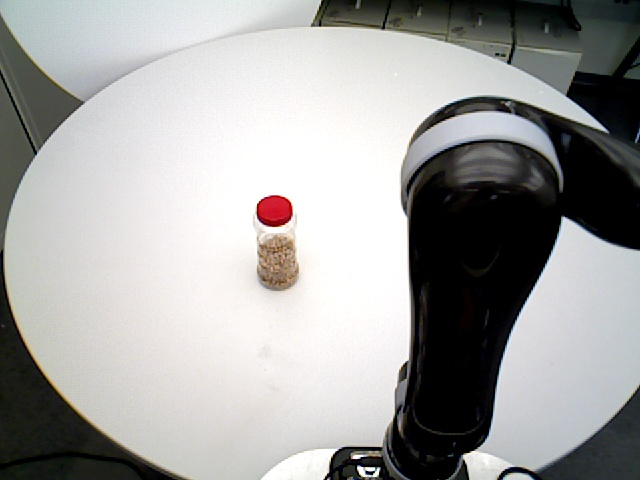
\includegraphics[scale=\examplepicsize]{figures/objects/23.JPG} & 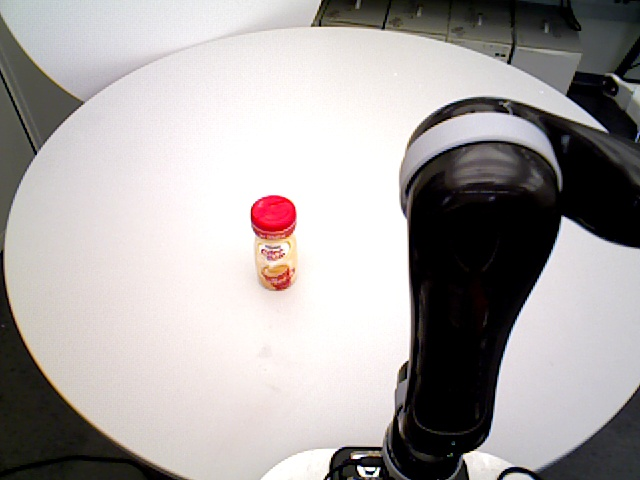
\includegraphics[scale=\examplepicsize]{figures/objects/17.JPG}\\ \hline
	\multicolumn{2}{|c|}{} & \multicolumn{6}{c|}{\bf vision only system} \\ \hline
	pink & -.3 & 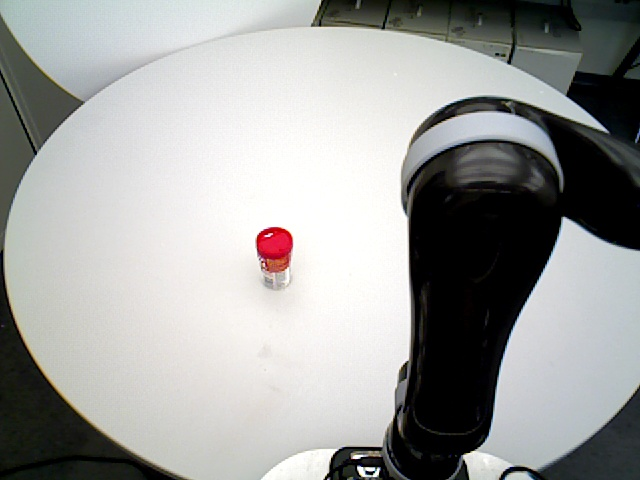
\includegraphics[scale=\examplepicsize]{figures/objects/11.JPG} & 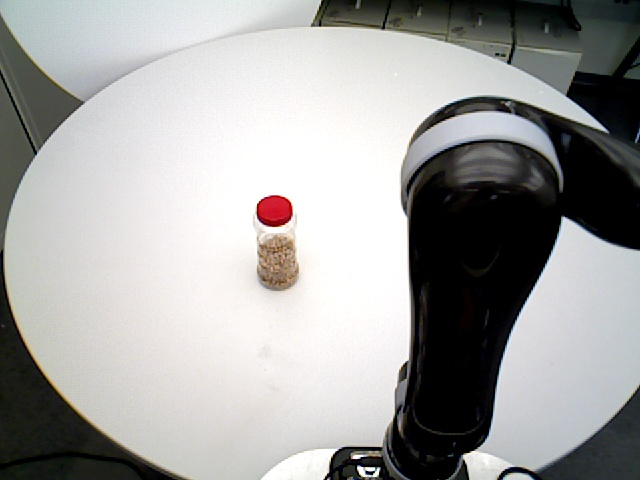
\includegraphics[scale=\examplepicsize]{figures/objects/23.JPG} & 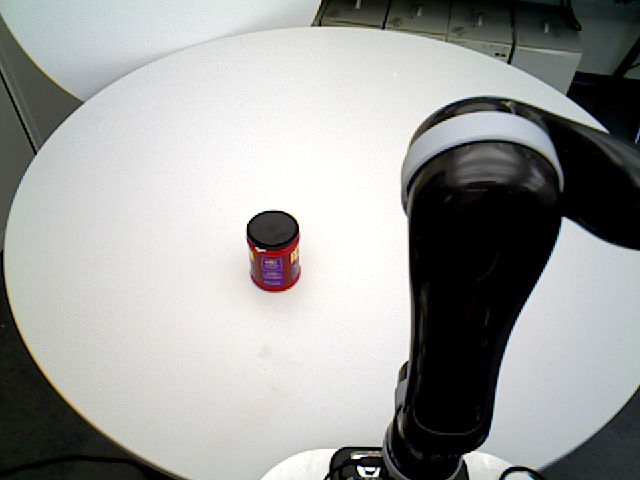
\includegraphics[scale=\examplepicsize]{figures/objects/10.JPG} & 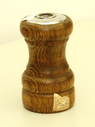
\includegraphics[scale=\examplepicsize]{figures/objects/8.JPG} & 
\includegraphics[scale=\examplepicsize]{figures/objects/2.JPG} & 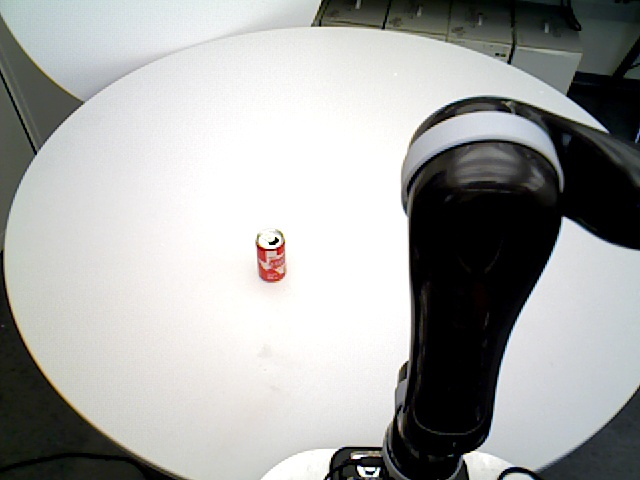
\includegraphics[scale=\examplepicsize]{figures/objects/27.JPG}\\ \hline
\end{tabular}
\caption{Predicates for which the difference $|f_1^{mm}-f_1^{vo}|$ between the \textbf{multi-modal} (mm) and \textbf{vision only} (vo) systems was greater than or equal to $0.3$, both systems had at least $10$ objects with labels for that predicate on which to train, and the system with the worse $f_1$ had at most 5 fewer objects with labels on which to train (to avoid rewarding a system just for having more training labels). The highest- and lowest-confidence objects for each predicate are shown. The top rows ($f_1^{mm}-f_1^{vo}>0$) are decisions from the \textbf{multi-modal} system, the bottom row from the \textbf{vision only} system.}
\label{tab:predicate_examples}
\end{table*}

The \textbf{multi-modal} system does well on the predicates ``tall'' and ``half-full'' which have non-visual interpretations.
A tall object will exert force earlier against the robot arm pressing down on it, while a half-full object will be lighter than a full one and heavier than an empty one.
The color predicate ``pink'' seems to confuse the multi-modal grounding system using non-visual information for this purely visual predicate.
This doesn't hold for ``yellow'', though the classifiers for ``yellow'' never became particularly good for either system.
For example, two of the three most confident objects in the multi-modal setting are false positives.

\textbf{Correlations to physical properties.} To validate whether the systems learned non-visual properties of objects, for every predicate we calculated the Pearson's correlation $r$ between its decision on each object and that object's measured weight, height, and width. 
As before, the decisions were made on held-out objects in leave-one-out cross validation.
We found predicates for which $r>0.5$ with $p<0.05$ when the system had at least $10$ objects with labels for the predicate on which to train.

The \textbf{vision only} system led to no predicates correlated against these physical object features.

The \textbf{multi-modal} system learned to ground predicates which correlate well to objects' height and weight.
The ``tall'' predicate correlates with objects that are higher ($r=.521$), ``small'' ($r=-.665$) correlates with objects that are lighter, and ``water'' ($r=.814$) correlates with objects that are heavier.
The latter is likely from objects described as ``water bottle'', which, in our dataset, are mostly filled either half-way or totally and thus heavier.
There is also a spurious correlation between ``blue'' and weight ($r=.549$).
This highlights the value of multi-modal grounding, since words like ``half-full'' cannot be evaluated with vision alone when dealing with closed containers that have unobservable contents.
